% This is "sig-alternate.tex" V2.0 May 2012
% This file should be compiled with V2.5 of "sig-alternate.cls" May 2012
%
% This example file demonstrates the use of the 'sig-alternate.cls'
% V2.5 LaTeX2e document class file. It is for those submitting
% articles to ACM Conference Proceedings WHO DO NOT WISH TO
% STRICTLY ADHERE TO THE SIGS (PUBS-BOARD-ENDORSED) STYLE.
% The 'sig-alternate.cls' file will produce a similar-looking,
% albeit, 'tighter' paper resulting in, invariably, fewer pages.
%
% ----------------------------------------------------------------------------------------------------------------
% This .tex file (and associated .cls V2.5) produces:
%       1) The Permission Statement
%       2) The Conference (location) Info information
%       3) The Copyright Line with ACM data
%       4) NO page numbers
%
% as against the acm_proc_article-sp.cls file which
% DOES NOT produce 1) thru' 3) above.
%
% Using 'sig-alternate.cls' you have control, however, from within
% the source .tex file, over both the CopyrightYear
% (defaulted to 200X) and the ACM Copyright Data
% (defaulted to X-XXXXX-XX-X/XX/XX).
% e.g.
% \CopyrightYear{2007} will cause 2007 to appear in the copyright line.
% \crdata{0-12345-67-8/90/12} will cause 0-12345-67-8/90/12 to appear in the copyright line.
%
% ---------------------------------------------------------------------------------------------------------------
% This .tex source is an example which *does* use
% the .bib file (from which the .bbl file % is produced).
% REMEMBER HOWEVER: After having produced the .bbl file,
% and prior to final submission, you *NEED* to 'insert'
% your .bbl file into your source .tex file so as to provide
% ONE 'self-contained' source file.
%
% ================= IF YOU HAVE QUESTIONS =======================
% Questions regarding the SIGS styles, SIGS policies and
% procedures, Conferences etc. should be sent to
% Adrienne Griscti (griscti@acm.org)
%
% Technical questions _only_ to
% Gerald Murray (murray@hq.acm.org)
% ===============================================================
%
% For tracking purposes - this is V2.0 - May 2012

\documentclass{sig-alternate}
\usepackage{placeins}
\begin{document}
%
% --- Author Metadata here ---
\conferenceinfo{SIGIR}{'15, August 9-13, 2015, Santiago, Chile}
%\CopyrightYear{2007} % Allows default copyright year (20XX) to be over-ridden - IF NEED BE.
%\crdata{0-12345-67-8/90/01}  % Allows default copyright data (0-89791-88-6/97/05) to be over-ridden - IF NEED BE.
% --- End of Author Metadata ---

\title{On the Construction of Ideal Query\\ for Patent Prior-art Search
%\titlenote{(Produces the permission block, and
%copyright information). For use with
%SIG-ALTERNATE.CLS. Supported by ACM.}
}
%\subtitle{Why Patent Prior-art Search Fails?
%\titlenote{A full version of this paper is available as
%\textit{Author's Guide to Preparing ACM SIG Proceedings Using
%\LaTeX$2_\epsilon$\ and BibTeX} at
%\texttt{www.acm.org/eaddress.htm}}
%}
%
% You need the command \numberofauthors to handle the 'placement
% and alignment' of the authors beneath the title.
%
% For aesthetic reasons, we recommend 'three authors at a time'
% i.e. three 'name/affiliation blocks' be placed beneath the title.
%
% NOTE: You are NOT restricted in how many 'rows' of
% "name/affiliations" may appear. We just ask that you restrict
% the number of 'columns' to three.
%
% Because of the available 'opening page real-estate'
% we ask you to refrain from putting more than six authors
% (two rows with three columns) beneath the article title.
% More than six makes the first-page appear very cluttered indeed.
%
% Use the \alignauthor commands to handle the names
% and affiliations for an 'aesthetic maximum' of six authors.
% Add names, affiliations, addresses for
% the seventh etc. author(s) as the argument for the
% \additionalauthors command.
% These 'additional authors' will be output/set for you
% without further effort on your part as the last section in
% the body of your article BEFORE References or any Appendices.

\numberofauthors{3} %  in this sample file, there are a *total*
% of EIGHT authors. SIX appear on the 'first-page' (for formatting
% reasons) and the remaining two appear in the \additionalauthors section.
%
\author{
% You can go ahead and credit any number of authors here,
% e.g. one 'row of three' or two rows (consisting of one row of three
% and a second row of one, two or three).
%
% The command \alignauthor (no curly braces needed) should
% precede each author name, affiliation/snail-mail address and
% e-mail address. Additionally, tag each line of
% affiliation/address with \affaddr, and tag the
% e-mail address with \email.
%
% 1st. author
\alignauthor
M O\\%\titlenote{Dr.~Trovato insisted his name be first.}\\
       \affaddr{NICTA \& ANU}\\
       \affaddr{Canberra, Australia}\\
       %\affaddr{Wallamaloo, New Zealand}\\
       \email{\scriptsize name.surname@nicta.com.au}
% 2nd. author
\alignauthor
W Z\\%\titlenote{The secretary disavows
%any knowledge of this author's actions.}\\
       \affaddr{NICTA \& ANU}\\
       \affaddr{Canberra, Australia}\\
       %\affaddr{Dublin, Ohio 43017-6221}\\
       \email{\scriptsize name.surname@nicta.com.au}
% 3rd. author
\alignauthor X Y\\%\titlenote{This author is the
%one who did all the really hard work.}\\
       \affaddr{NICTA \& ANU}\\
       \affaddr{Canberra, Australia}\\
      % \affaddr{Hekla, Iceland}\\
       \email{\scriptsize name.surname@nicta.com.au}
%\and  % use '\and' if you need 'another row' of author names
% 4th. author
%\alignauthor Lawrence P. Leipuner\\
%       \affaddr{Brookhaven Laboratories}\\
%       \affaddr{Brookhaven National Lab}\\
%       \affaddr{P.O. Box 5000}\\
%       \email{lleipuner@researchlabs.org}
% 5th. author
%\alignauthor Sean Fogarty\\
%       \affaddr{NASA Ames Research Center}\\
%       \affaddr{Moffett Field}\\
%       \affaddr{California 94035}\\
%       \email{fogartys@amesres.org}
%% 6th. author
%\alignauthor Charles Palmer\\
%       \affaddr{Palmer Research Laboratories}\\
%       \affaddr{8600 Datapoint Drive}\\
%       \affaddr{San Antonio, Texas 78229}\\
%       \email{cpalmer@prl.com}
}
% There's nothing stopping you putting the seventh, eighth, etc.
% author on the opening page (as the 'third row') but we ask,
% for aesthetic reasons that you place these 'additional authors'
% in the \additional authors block, viz.
%\additionalauthors{Additional authors: John Smith (The Th{\o}rv{\"a}ld Group,
%email: {\texttt{jsmith@affiliation.org}}) and Julius P.~Kumquat
%(The Kumquat Consortium, email: {\texttt{jpkumquat@consortium.net}}).}
\date{30 July 1999}
% Just remember to make sure that the TOTAL number of authors
% is the number that will appear on the first page PLUS the
% number that will appear in the \additionalauthors section.

\maketitle
\begin{abstract}
Patent prior-art search aims to find all relevant patents which may invalidate the novelty of a patent application or at least have common parts with patent application and should be cited. Patent search has been the centre of attention in IR communities for years, however it has lower retrieval effectiveness compared to other IR applications. In this work, we focused on the causes of failure rather than solutions. We started with relevance feedback to get a golden standard, then we concentrated on heuristics correlate with our RF standard. Finally, we showed that features other than relevance feedback can not be helpful because they are a complex mixture of useful words and noisy words. Finally, we got a considerable improvement by user feedback with a minimum effort.      
 
\end{abstract}

% A category with the (minimum) three required fields
\category{H.3.3}{Information Search and Retrieval}{Query Formulation}
%A category including the fourth, optional field follows...
%\category{D.2.8}{Software Engineering}{Metrics}[complexity measures, performance measures]

%\terms{Theory}

\keywords{Patent search, Query Reformulation, Data Analysis}

\section{Introduction}
%A patent is a set of exclusive rights granted by a sovereign state to an inventor for a limited period of time to encourage detailed public disclosure of new technologies and novel ideas. An important requirement for a patent to be granted is that the invention, it describes, is novel which means there is no earlier patent, publication or public communication of a similar idea. To ensure the novelty of an invention, patent offices as well as other Intellectual Property (IP) service providers mainly perform a search called 'prior art search'. The purpose of 'prior art search' is finding all relevant patents which may put the patent application at the risk of novelty invalidation or at least have common parts with patent application and should be cited~\cite{Magdy2012}~\cite{piroi2013overview}. 
A patent is a set of exclusive rights granted to an inventor to protect their invention for a limited period of time. An important requirement for a patent to be granted is that the invention, it describes, is novel which means there is no earlier patent, publication or public communication of a similar idea. To ensure the novelty of an invention, patent offices as well as other Intellectual Property (IP) service providers mainly perform a search called `prior art search'. The purpose of `prior art search' is finding all relevant patents which may put the patent application at the risk of novelty invalidation or at least have common parts with patent application and should be cited~\cite{magdy2012toward}~\cite{piroi2013overview}. 

Patent retrieval has three main characteristics which makes it difficult compared to other IR applications: the search starts with a query as long as a full patent application that helps users --usually patent examiners, inventors, or lawyers-- avoid spending long hours to formulate a query; it is recall-oriented, where not missing relevant documents is more important than appearing relevant documents at top of the list; unlike the web application in which authors tend to highlight their work to be easily found through search engines, authors of the patents prefer to use a vague language to avoid the invalidation of their idea.     

Many works has been conducted to improve the patent retrieval effectiveness so far. However, either the results showed quite small improvement or the proposed methods were complicated and computationally expensive. Overall, the works on patent search fall in five main categories: query reformulation(query expansion and query reduction), query term selection, query suggestions, using patent meta-data and images for retrieval~\cite{lupu2013evaluating}, and Cross-Language Information Retrieval~\cite{magdy2014studying}.

%Applying standard information retrieval (IR) techniques to patent search is not effective and needs applying supplementary methods to improve the effectiveness. Although lots of methods have been proposed in recent years, reported results for different tasks of patent search show lower retrieval effectiveness compared to other IR applications~\cite{lupu2013patent}.  
In this work, we mainly emphasized on the problem from the data analysis perspective rather than the solution, since the results, reported in the previous works, are lower than the performance for the other IR applications. We started with relevance feedback to find a golden standard for our analysis, then we examined possible recognized features to find a heuristic that correlate with our relevance feedback results. We avoided complex feature which are computationally expensive such as Pair-wise Term Proximity features~\cite{bashir2010improving}. Finally, we could double the `MAP' with the minimum user effort. 
\section{Baseline IR System}
%\subsection{Experimental Setup}
We developed a Lucene-based%
\footnote{\texttt{http://lucene.apache.org/}%
} IR system with the possibility of using diverse generic IR models: TF-IDF, BM25, Language Models(Dirichlet smoothing, and Jelinek-Mercer smoothing) as our baseline system. We achieved the best baseline effectiveness using the `Description' of the patent application as a query\cite{xue2009transforming}, and Language Model with Dirichlet smoothing as a retrieval model. We conducted our experiments on CLEF-IP%
\footnote{\texttt{\url{http://www.ifs.tuwien.ac.at/~clef-ip/}}}% 
 2010 data collection, with 2.6 million European patent documents and 1303 English topics(queries). On the collection side, we only indexed English subset of each section of a patent (title, abstract, claims, and description), and IPC\footnote{International Patent Classification}% 
  code in a separate field\cite{magdy2012toward}. We also used the patent classification assigned to the query topics to filter search results to match at least one of the query IPC codes\cite{lopez2010patatras}. Our experiments showed that using IPC filter is itself a source of error because about 19\% of relevant patents in CLEF-IP data collection do not share any classification code with their query. However, for our analysis, we kept the filter on since it makes the matching process between the query and documents notably faster.
 %\footnote{\texttt{For an accurate term analysis, we pruned out the source of errors related to data curation such as non-English patents, and IPC filter.}%
%}.
\begin{figure*}
\begin{center}
\noindent\begin{minipage}[b]{0.3\linewidth}
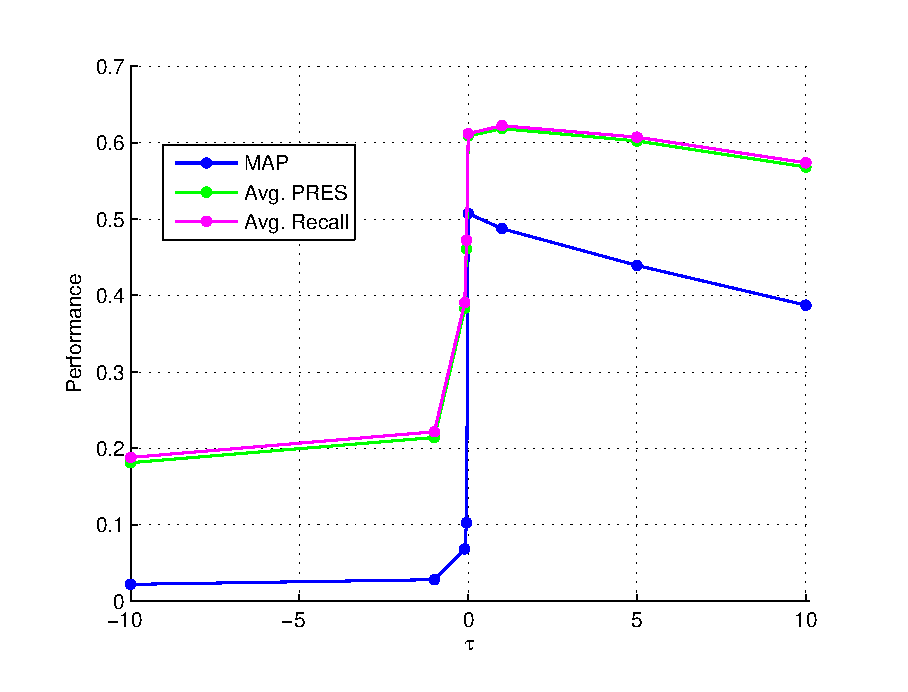
\includegraphics[width=\linewidth]{figs/extended-optquery-tau.eps}
\end{minipage}%
\hfill
%\hspace{7mm}
\begin{minipage}[b]{0.3\linewidth}
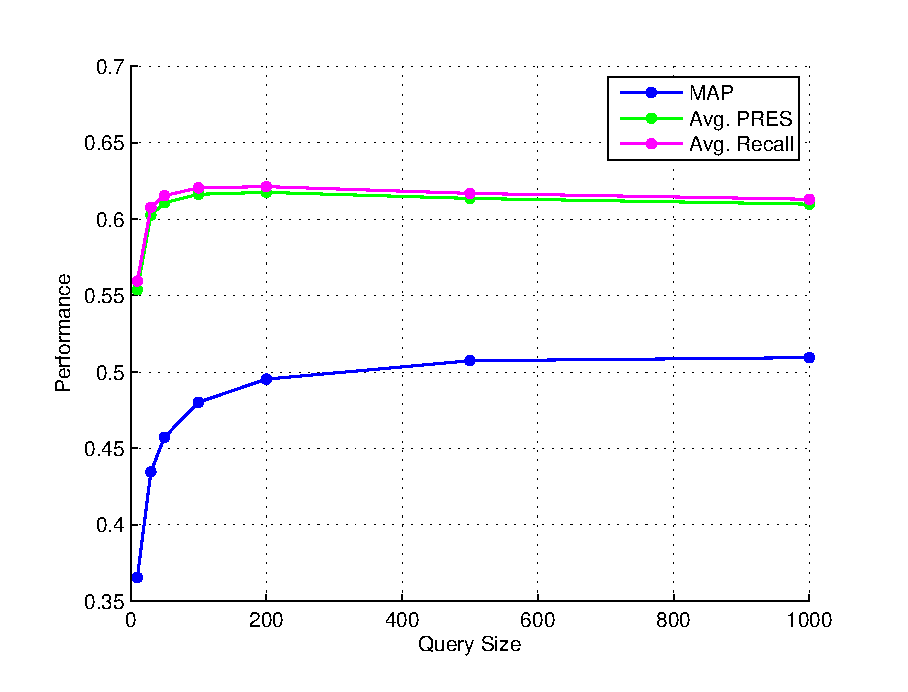
\includegraphics[width=\linewidth]{figs/opt-query-qsize.eps}
\end{minipage}
%\vspace{-3mm}\\
%(a) \hspace{30mm}(b)\\
\hfill
%\hspace{7mm}
\begin{minipage}[b]{0.3\linewidth}
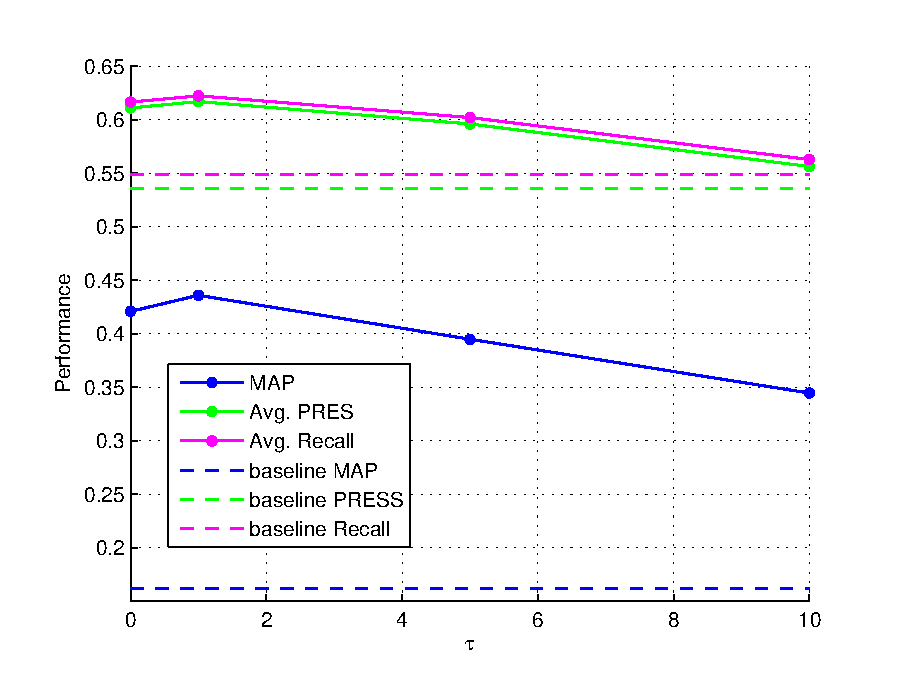
\includegraphics[width=\linewidth]{figs/opt-patentquery-tau.eps}
\end{minipage}
\vspace{-0.5mm}\\
 \hspace{2mm}(a) \hspace{55mm}(b) \hspace{58mm} (c)
\caption{\footnotesize
How score threshold($\tau$) and query size controls the performance.
(a) Performance versus the score threshold. (b) Performance versus the query size. (c) System performance when we reduced the query by RF: $ query = Q\cap (useful \; terms) $, where $ Q $ is the patent query and $ useful\; terms = \{t| score_{RF}(t)>\tau\} $.}
\vspace{-4mm}
\end{center}
\label{fig:control}
\end{figure*}
\section{Ideal Query}
The main complain about patent search is insufficient match between the content of patent queries and relevant
patents\cite{lupu2013patent}\cite{magdy2012toward}. However, we have the intuition that there are sufficient terms in a patent query containing thousands words to be matched with the relevant patents. So, in this section, we focused on term analysis to figure out the main causes that the system fails in retrieving relevant documents at top of the result list. 

We started our analysis using {\em relevance feedback}, in which the user gives feedback on the relevance of documents in an initial set of results to improve the final result set. We calculate a relevance feedback(RF) score for each term in top-100 retrieved documents as follows:
\begin{equation}
score_{RF}(t,Q)=Rel(t)-Irr(t) 
 \label{eq:score}
\end{equation}\vspace*{-5ex}
\begin{displaymath}t\in \lbrace \mbox{terms in top-100 retrieved documents}\rbrace\end{displaymath}
where $ Rel(t) $ is the average term frequency in retrieved relevant patents and $ Irr(t) $ is the average term frequency in retrieved irrelevant patents. We assumed that words with a positive score are {\em useful words} since they are more frequent in relevant patents, while words with negative score are {\em noisy words} as they appear more frequently in irrelevant patents. 

We expected to see a higher performance for the queries which contain more {\em useful words}, but, surprisingly, we could not find any correlation between the performance and the percentage of {\em useful words} in the query. 

\subsection{Ideal Query Formulation}
We hypothesized that a query, formulated by only the {\em useful terms}, is the best possible query we can make since they are all frequent in relevant patents but rare in irrelevant ones. We formulated the ideal query as follows: 
\begin{equation}
Ideal\; query = \{t \in top-100|score_{RF}(t)>0\}   
 \label{eq:score}
\end{equation}
Table \ref{tab:optquery} compares the baseline performance, where the query is the full patent application, with the performance of the ideal query. 
\begin{table}[htpb]
  \begin{center}
   \caption{System performance for the baseline and ideal query.}
  \input table/optquery.tex   
  \label{tab:optquery}
  \end{center}  
\end{table}
It can be seen that MAP jumps from 0.1618 to {\em 0.5075}, which means the ideal query considerably performs better than the baseline. Hence, we used it as a golden standard. 
\subsection{Patent Query and Useful Terms}
Our previous experiments led us to the hypothesis that a patent query contains sufficient words matched with the relevant patents.
% and the {\em noisy words} are the main cause of the low effectiveness. 
To prove our idea, we formulated a query by selecting only RF {\em useful terms} existing inside patent query as follows: 
\begin{equation}
 query = \{t|t \in \{ Q\cap (useful \; terms)\}\}   
 \label{eq:score}
\end{equation}
The results were encouraging, as MAP was improved from 0.1618 to {\em 0.44}.
\subsection{Analyse the Results}
The main results related to ideal query formulation has summarized in Figure 1. 

Fig. (1-c) explicitly shows that a patent query contains sufficient words to retrieve relevant patents at top of the list. We only need to keep the {\em useful terms} and prune out the {\em noisy words}.

We use a score threshold($\tau$) to formulate the RF query (we select the terms with $ score(t)>\tau $). 
%Fig. 1 indicates how the score threshold and the query size control the performance. 
%\begin{figure}[htpb]
%\centering
%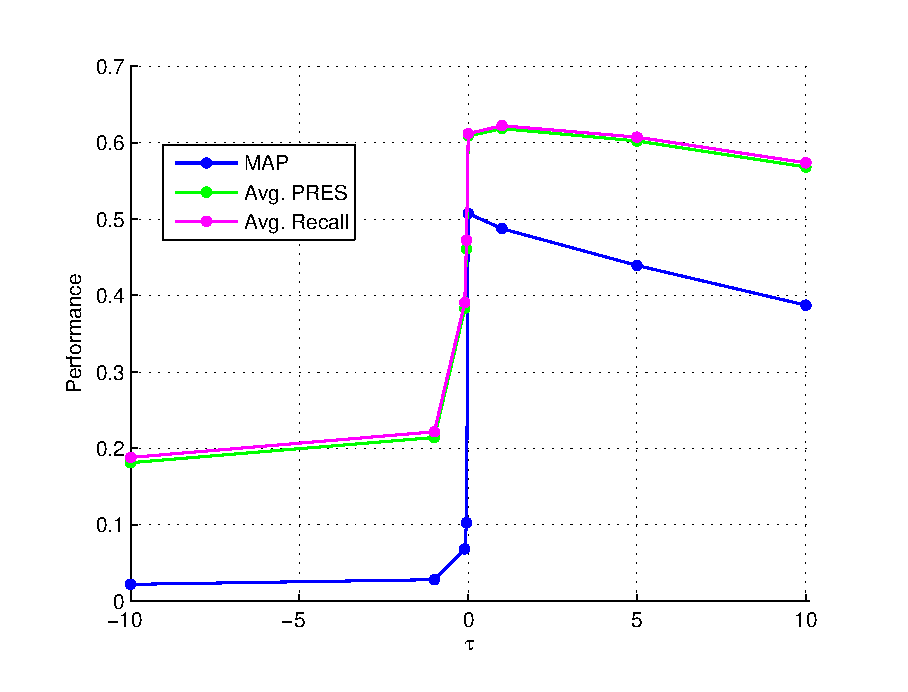
\epsfig{file=figs/extended-optquery-tau.eps, height=2in, width=3.1in}
%\caption{A sample black and white graphic (.eps format).}
%\end{figure}

%\FloatBarrier
Fig. (1-a) indicates two important facts. First, it shows that the performance decreases by increasing the threshold which means all words with a positive score are helpful for the performance. Second, the system is over-sensitive to the {\em noisy words}($ \tau<0 $). Fig. (1-b) shows that formulating a query with up to 200 {\em useful words} helps performance whereas there is no significant improvement by adding more than 200 words. 
%\begin{figure}[htpb]
%\begin{center}
%\noindent\begin{minipage}[b]{0.5\linewidth}
%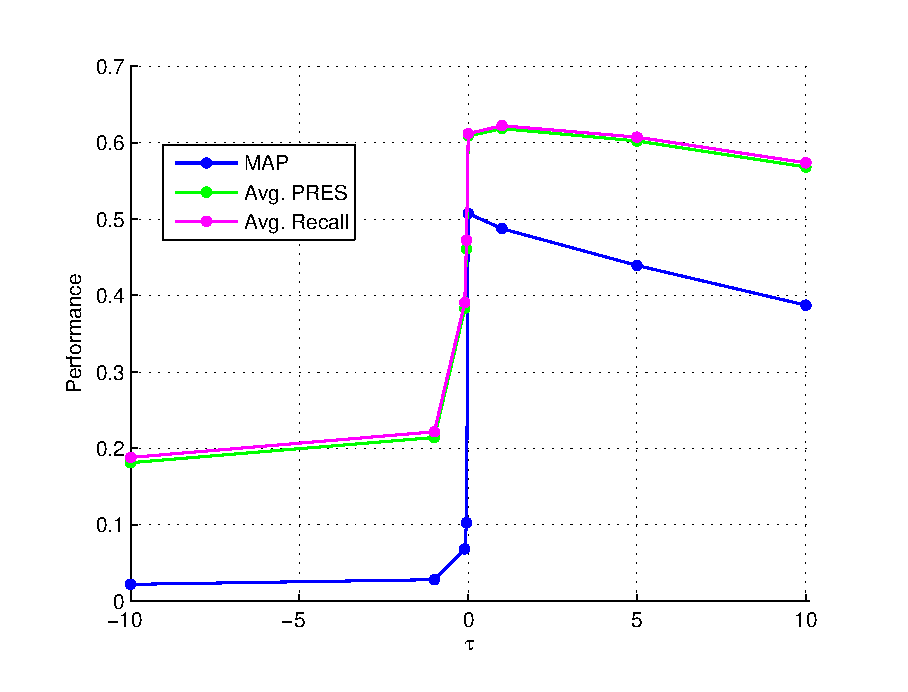
\includegraphics[width=\linewidth]{figs/extended-optquery-tau.eps}
%\end{minipage}%
%\hfill
%%\hspace{7mm}
%\begin{minipage}[b]{0.5\linewidth}
%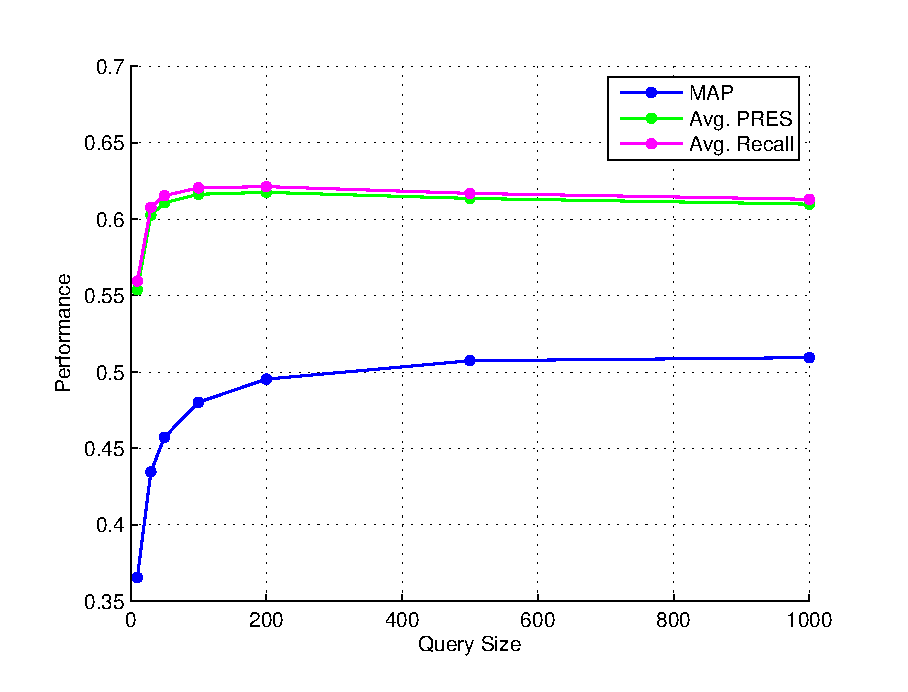
\includegraphics[width=\linewidth]{figs/opt-query-qsize.eps}
%\end{minipage}
%\vspace{-3mm}\\
%(a) \hspace{30mm}(b)\\
%%\hfill
%%\hspace{7mm}
%\begin{minipage}[b]{0.5\linewidth}
%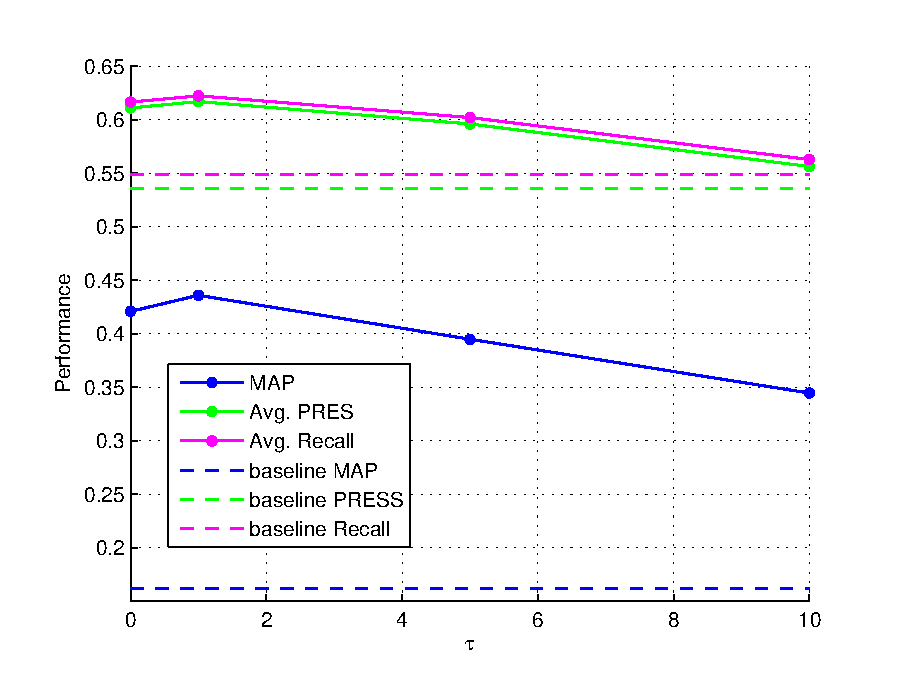
\includegraphics[width=\linewidth]{figs/opt-patentquery-tau.eps}
%\end{minipage}
%\vspace{-3mm}\\
%(c)
%\caption{\footnotesize
%How score threshold($\tau$) and query size controls the performance.
%(a) Performance versus the score threshold. (b) Performance versus the query size. (c) System performance when we reduced the query by RF: $ query = Q\cap (useful \; terms) $, where $ Q $ is the patent query and $ useful\; terms = \{t| score_{RF}(t)>\tau\} $.}
%\label{fig:mom2}
%\vspace{-4mm}
%\end{center}
%\label{fig:control}
%\end{figure}


%\begin{figure}[htpb]
%   \centering
%   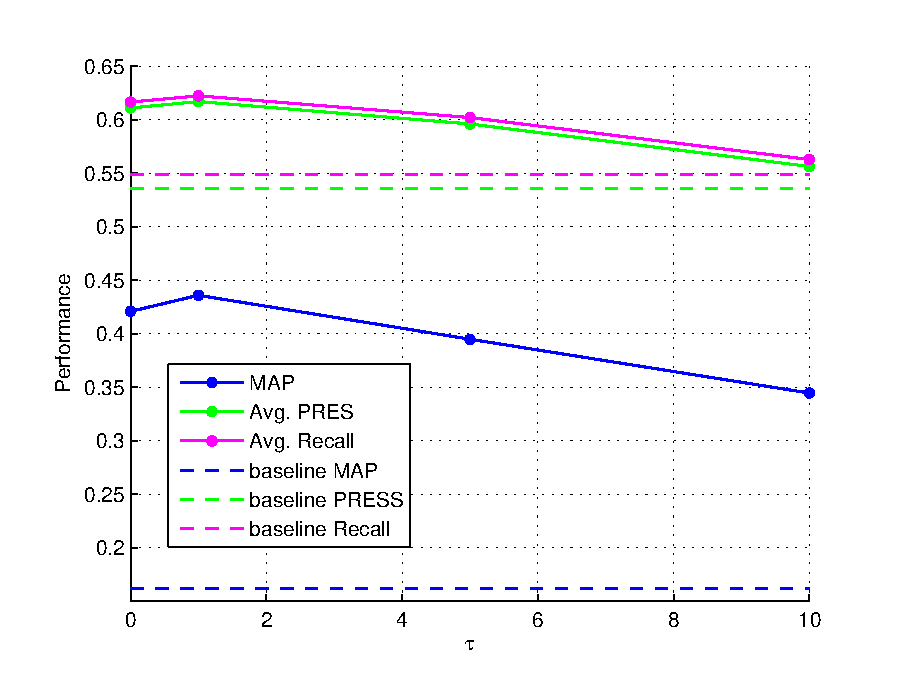
\includegraphics[width=0.3\textwidth,height=35mm]{figs/opt-patentquery-tau.eps}
%   \caption{Optimal patent query performance vs. score threshold of useful terms to select patent query terms. $ query = Q\cap (useful \; terms) $, where $ Q $ is the patent query and $ useful\; terms = \{t| score_{RF}(t)>\tau\} $..}   
%   \label{fig:optpatentquery} 
%\end{figure}

\section{Standard Methods for Query Reduction}
We achieved a notable improvement in performance using relevance feedback, however, it will cost to have a relevance feedback from our users who are professional patent examiners. For this reason, we considered the relevance feedback as a {\em golden standard} and focused to recognize the other accessible features that correlate with RF score. The most obvious accessible elements in our patent search engine are: patent query, top-100 patent documents retrieved in the first retrieval (features such as document frequent(DF) words and PRF words), and IPC code definition words.  
\subsubsection{Identify the Noisy Words}
We showed that there are sufficient useful terms in a patent query(Fig. 1-c) to achieve good results but additional words which are considered noise are the main cause of low effectiveness. We hypothesized that the noisy words are frequent in top-100 retrieved documents and we can refine the query by removing document frequent words from the patent query. We calculated document frequent score for each term in top-100 retrieved patent documents as follows:
\begin{equation}
score_{DF}(t)= \frac{1}{100}\sum_{t\in \lbrace Top-100\rbrace} TF(t)  
 \label{eq:dfscore}
\end{equation}
where TF(t) is term frequency of each word. 
\begin{figure}[htpb]
\begin{center}
\noindent\begin{minipage}[b]{0.52\linewidth}
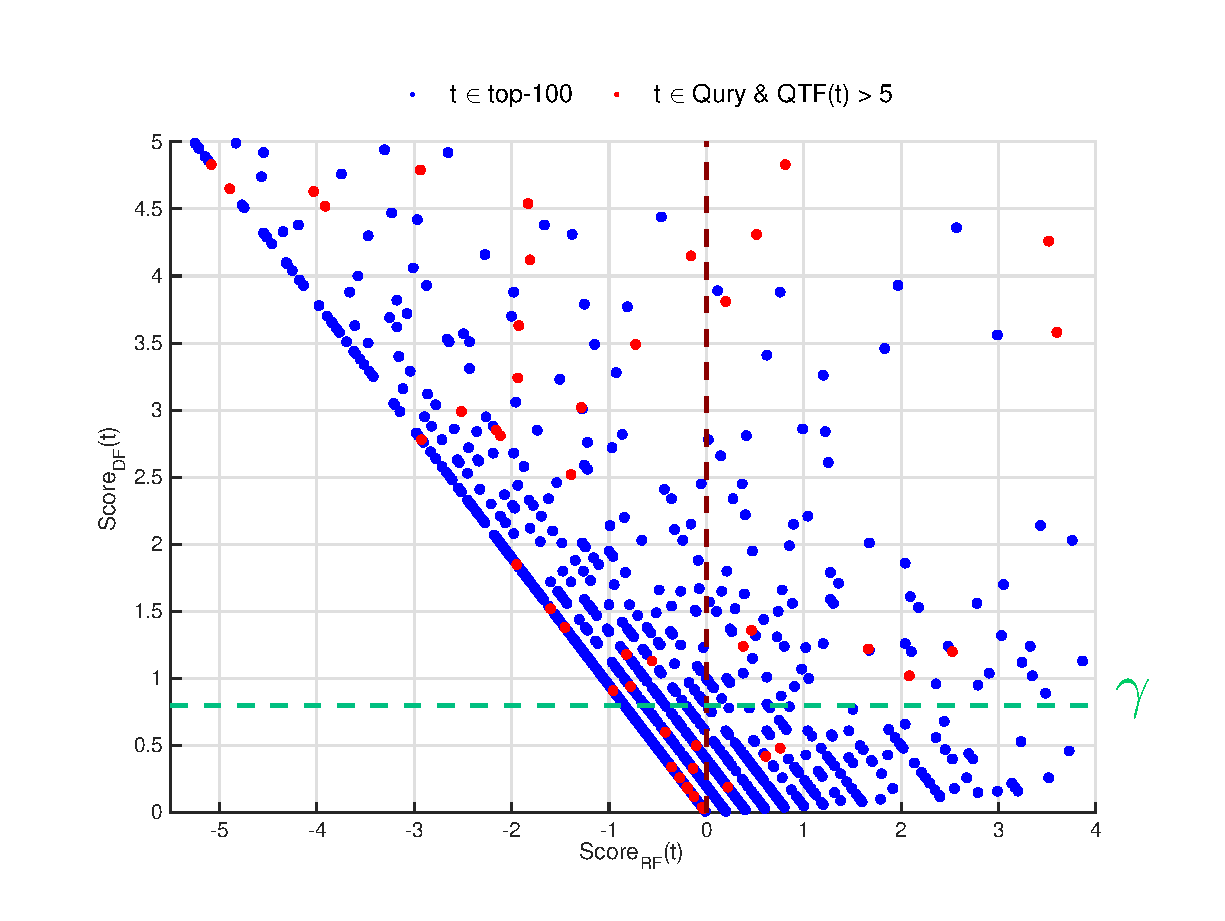
\includegraphics[width=\linewidth]{figs/df-rf-tauline.eps}
\end{minipage}%%%%%%%%%%%
\hfill
%\hspace{7mm}
\begin{minipage}[b]{0.48\linewidth}
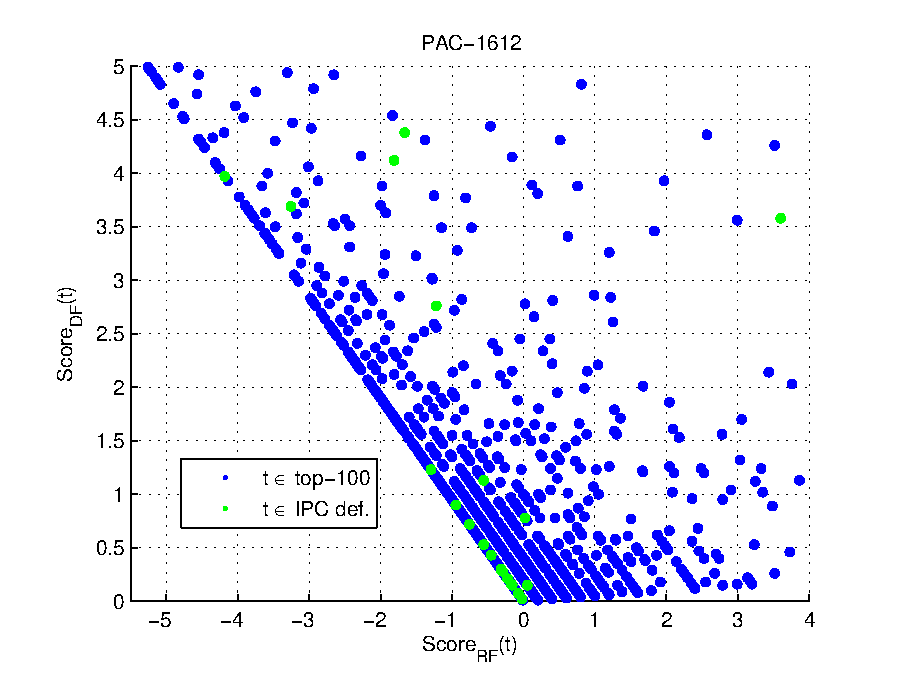
\includegraphics[width=\linewidth]{figs/ipcdef-rf-df.eps}
\end{minipage}
%\vspace{-3mm}\\
%(a) \hspace{30mm}(b)\\
%\hfill
%%\hspace{7mm}
%\begin{minipage}[b]{0.3\linewidth}
%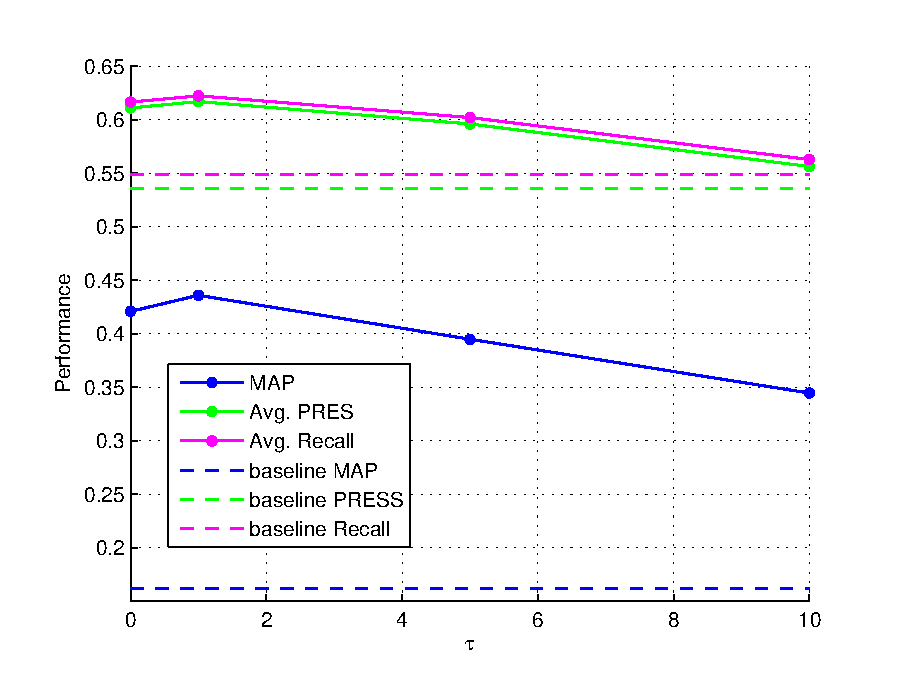
\includegraphics[width=\linewidth]{figs/opt-patentquery-tau.eps}
%\end{minipage}
\vspace{-4mm}\\
 \hspace{5mm}(a) \hspace{38mm}(b) 
\caption{\footnotesize
Anecdotal example: Scatter plot of $ score_{RF}(t) $ versus $ score_{DF}(t) $ for the words in top-100 retrieved documents. Each blue point is a vocabulary in top-100 retrieved document vocabulary set. (a) Points highlighted in red are query words with term frequency higher than 5($ QTF(t)>5 $) and (b) points in green are IPC definition words.}
\vspace{-4mm}
\end{center}
\label{fig:dfrf}
\end{figure}
 %\vspace*{-2ex}
%\begin{figure}[htpb]
%   \centering
%   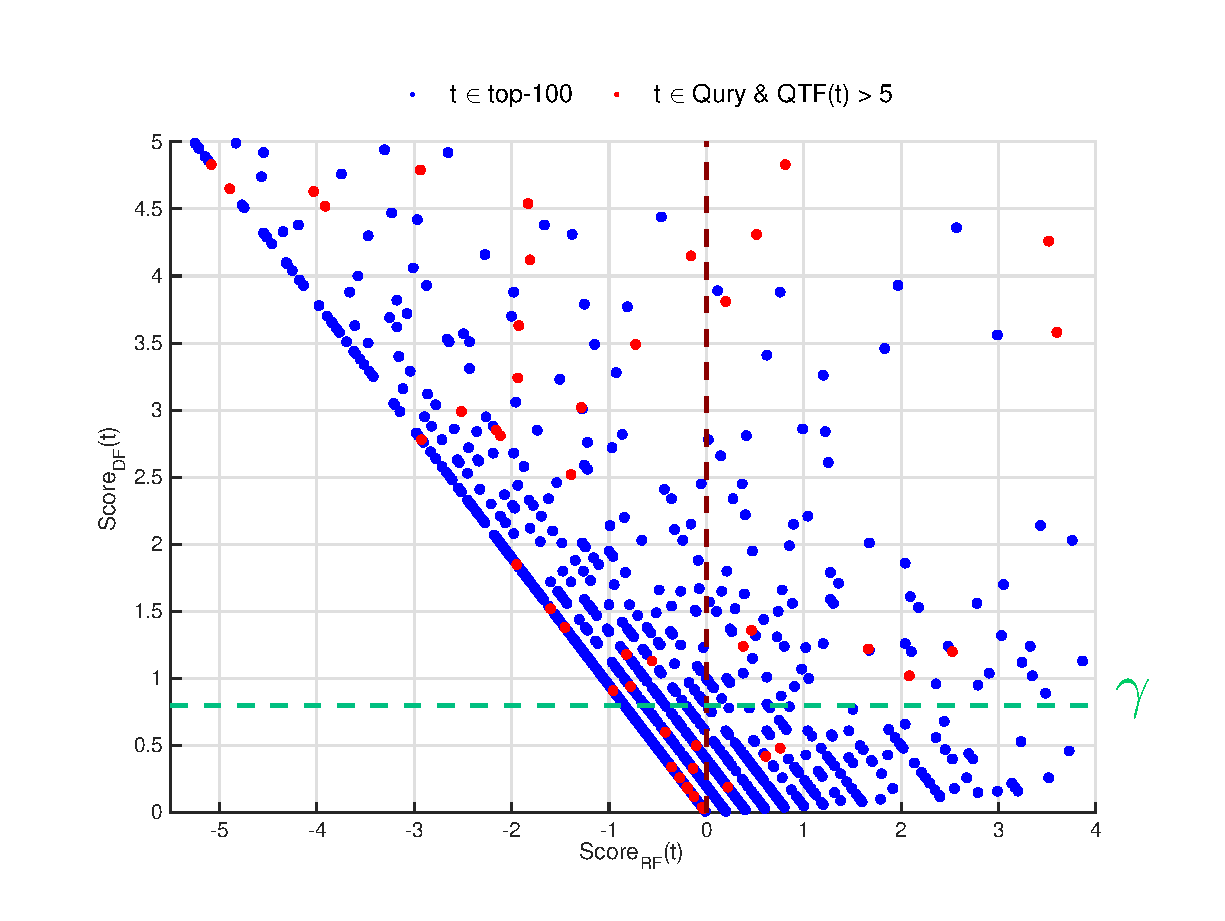
\includegraphics[width=0.30\textwidth,height=40mm]{figs/df-rf-tauline.eps}
%   \caption{Anecdotal example: Scatter plot of $ score_{RF}(t) $ versus $ score_{DF}(t) $ for the words in top-100 retrieved documents. Each blue point is a vocabulary in top-100 retrieved document vocabulary set. Points highlighted in red are query words with term frequency higher than 5($ QTF(t)>5 $).}   
%   \label{fig:dfrf} 
%\end{figure}
Fig. 2 shows a scatter plot of RF score and DF score of words in top-100 retrieved patents. A negative correlation shows that these two scores have opposite trends. Fig. 2-a is divided into four areas: 
(a) $score_{DF}(t)>\gamma$ and $score_{RF}(t)<0$ 
(b) $score_{DF}(t)>\gamma$ and $score_{RF}(t)>0$ 
(c) $score_{DF}(t)<\gamma$ and $score_{RF}(t)<0$
(d) $score_{DF}(t)>\gamma$ and $score_{RF}(t)>0$. 
If we remove the words with a DF score higher than a threshold($score_{DF}(t)>\gamma$), we will remove noisy words of the area `a' and keeping useful terms in area `d' which is desirable. Whereas, the areas `b' and `c' are not desirable because many noisy words are kept in area `c' while useful terms are removed from area `b'. To keep useful terms in area `b', we added the second condition to remove DF words while keeping query terms with a term frequency higher than a threshold $\delta$ ($ score_{DF}(t)<\gamma \mbox{ \& } QTF(t)>\delta$). Even the best result, obtained with the $ \gamma = 0.01 $ and $ \delta = 5 $, could not beat the baseline. If we remove document frequent words but keep query words with term frequency higher than 5(highlighted with red in Fig. 2), we are still keeping sufficient amount of noisy words which are also frequent in the query to destroy the retrieval effectiveness. 

To remove the noisy words which are both frequent in retrieved documents and query, we considered the third feature: IPC code definition. IPC code definition are short sentences giving a general description about the topic that each patent belongs to. In almost all queries IPC code definition words have a negative RF score but few with positive RF scores(Fig. 2-b). Our experiments showed that adding the third condition to remove frequent query word that is in IPC code definition words deteriorated the performance which means removing even just few useful words in patent query can be destructive.     
%(a)(b)(c (d)\\
%Removing words with the $score_{DF}(t)>\gamma$  from the patent query is desirable for the words with $ score_{RF}(t)<0 $ while it is not desired for the words with the $ score_{RF}(t)>0 $. On the other hand, keeping noisy words is harm    
\subsubsection{Pseudo Relevance Feedback(PRF)}
The main advantage of pseudo relevance feedback or a blind feedback is that it is an automated process without user interaction which assumes the top k ranked documents are relevant and the others are irrelevant. It has been found to improve performance in many applications, however it did not worked in patent prior-art search. The results for PRF query formulation and query term selection using PRF were below the baseline. In fact, we could not find any heuristic correlates between  $ score_{RF}(t)$ and $ score_{PRF}(t)$. Fig. \ref{fig:anecdotal} explains the reason; it is an anecdotal example of a sample query with its abstract and a pair of PRF terms, with $ score_{PRF}(t)>10 $, and RF score of each term. It can be seen that terms with high PRF score are considered noise since their RF score is negative. Fig. \ref{fig:anecdotal} combined with Fig. 1-a can justify that terms from PRF are not useful at all because they contain sufficient noisy words to destruct the retrieval effectiveness. 
\begin{figure}[htpb]
\begin{framed}
\vspace*{-2ex}
  \centering
    %\lstinputlisting[frame=single, basicstyle=\scriptsize\ttfamily , linewidth=\columnwidth,breaklines=true]{code/anecdotale.tex}\vspace*{-2ex}
 \begin{lstlisting}[basicstyle=\tiny\ttfamily , linewidth=\columnwidth,breaklines=true] 
PAC-1612
Abstract: A wireless communication method for transmitting data from at least one master to one or more slaves positioned at various spatial locations and configured for generally simultaneous reception of the data. The method includes dividing the data into a number of portions, transmitting at least some of the portions using different transmission configurations for the different portions, having one or more of the slaves measure the quality of transmission associated with the group of different transmission configurations, and processing the quality measurements to determine new transmission configurations for use in transmitting the data.

PRF Terms: <@\textcolor{red}{commun:-69.43159}@>, <@\textcolor{red}{transmiss:-58.168427}@>, <@\textcolor{red}{wireless:-7.68421}@>, <@\textcolor{red}{telephon:-25.17895}@>, <@\textcolor{red}{recept:-37.810528}@>, <@\textcolor{red}{slave:-31.0421}@>, <@\textcolor{red}{deleg:-22.368422}@>, <@\textcolor{red}{turn:-18.536846}@>, <@\textcolor{red}{master:-35.778954}@>, <@\textcolor{red}{origin:-4.7473674}@>, <@\textcolor{blue}{schedul:12.852628}@>, <@\textcolor{red}{control:-14.842104}@>, <@\textcolor{blue}{frequenc:60.34737}@>, <@\textcolor{red}{station:-76.26316}@>, <@\textcolor{red}{electron:-8.442106}@>, <@\textcolor{red}{perform:-9.71579}@>, <@\textcolor{blue}{band:16.789476}@>, <@\textcolor{red}{termin:-40.04211}@>, <@\textcolor{blue}{indic:3.6210496}@>, <@\textcolor{red}{reason:-6.642107}@>, <@\textcolor{red}{apparatus:-6.2421055}@>, <@\textcolor{red}{determin:-8.97895}@>, <@\textcolor{red}{complet:-8.842103}@>, <@\textcolor{red}{prohibit:-3.8947372}@>, <@\textcolor{red}{state:-9.557897}@>, <@\textcolor{blue}{link:1.1157892}@>, <@\textcolor{blue}{hop:24.378946}@>, <@\textcolor{red}{lan:-8.3368435}@>, <@\textcolor{red}{assign:-9.68421}@>, <@\textcolor{blue}{f1:14.926317}@>, <@\textcolor{red}{short:-3.6000004}@>, <@\textcolor{blue}{pattern:17.58947}@>, <@\textcolor{blue}{paramet:1.5473672}@>, <@\textcolor{red}{serv:-4.5684214}@>, <@\textcolor{blue}{permit:0.62105286}@>
 \end{lstlisting} 
 \vspace*{-2ex}
\end{framed}
 \vspace*{-2ex}
  \caption{Anecdotal example: it shows the abstract and $ PRF \; term: \; score_{RF}(PRF \; term) $ pair of a sample query. Useful terms are highlighted in blue and the noisy ones in red.}
  \label{fig:anecdotal}  
\end{figure}
%\vspace*{-2ex}

Surprisingly, there were no pattern or correlation between accessible features and RF score and we could not refine the patent query with just useful terms as what we could with relevance feedback. 
\section{Improved by Minimum User Effort}
All our attempts to improve the system effectiveness without accessing the relevance feedback were quite in vein because the features we recognized were tightly the combination of the useful words and noisy words and the system performance is too sensitive to the existence of a noisy word or the absence of the useful terms. So, we decided to involve the users but with the least effort. In this experiment, we selected the query words using merely the few first-ranked relevant patents. Table \ref{tab:firstrel} shows that we can double the 'MAP' by only the first-ranked relevant document.
\begin{table}[htpb]
  \begin{center}
   \caption{System performance when only the first relevant patent used for query reduction. $\tau$ is RF score threshold, and $k$ indicates the number of first relevant retrieved documents.}\vspace{3mm}
  \input table/partialRFtermselect.tex   
  \label{tab:firstrel}
  \end{center}  
\end{table}
 We hypothesised that recognising the first-ranked patent is easy for a patent examiner because we expected that it appears at top-5 in first retrieval. Fig. \ref{fig:FirstTPRankHisto} confirms our intuition; The probability of finding the first-ranked relevant document at top-5 is acceptably high.   
\begin{figure}[htpb]
   \centering
   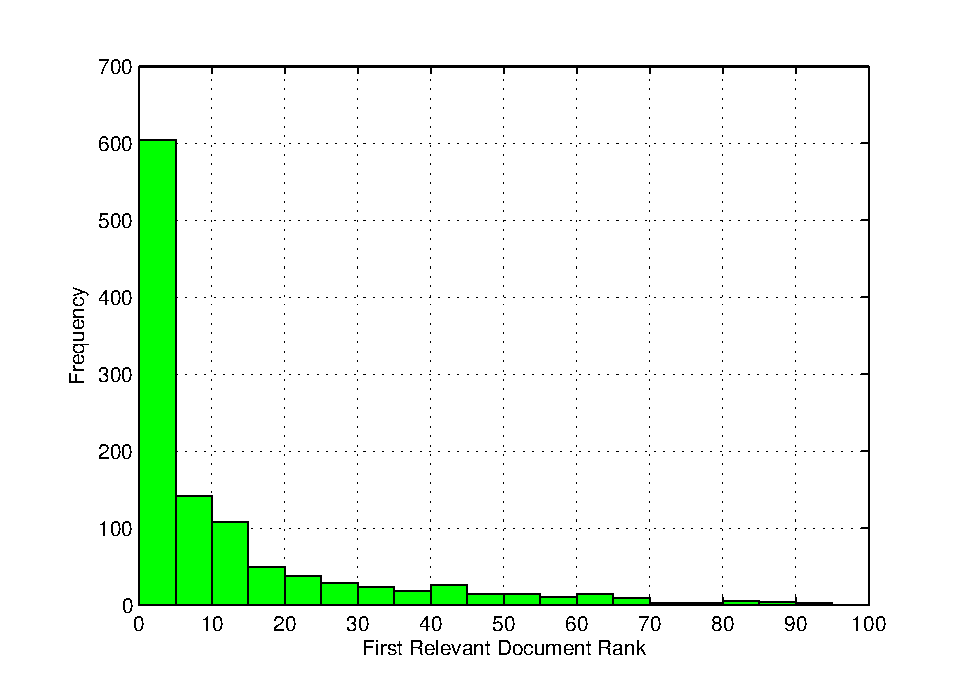
\includegraphics[width=0.25\textwidth,height=32mm]{figs/FirstTPRank.eps}
   \caption{The distribution of the first relevant document rank over test queries which have TPs}   
   \label{fig:FirstTPRankHisto} 
\end{figure}
%\section{Related Work}
\section{Related Work}
Our work is different from pioneer studies on patent retrieval, as we closely looked into the problem rather than solutions to figure out the causes that generic IR models which are based on term matching process, do not work efficiently in patent domain. Magdy et al.~\cite{magdy2011study} studied works on query expansion in patent retrieval and discussed that standard query expansion techniques are less effective, where the initial query is the full texts of query patents. Mahdabi et al.~\cite{Mahdabi2013} used term proximity information to identify expansion terms. Ganguly et al.~\cite{ganguly2011patent} adapted pseudo relevance feedback for query reduction by decomposing a patent application into constituent text segments and computing the Language Modelling (LM) similarities of each segment from the top ranked documents. The least similar segments to the pseudo-relevant documents removed from the query, hypothesizing it can increase the precision of retrieval. Kim et al.~\cite{kim2014diversifying} provided diverse query suggestion using aspect identification from a patent query to increase the chance of retrieving relevant documents. Mahdabi et al.~\cite{mahdabi2014patent} used linked-based structure of the citation graph together with IPC classification --the most useful patent meta-data-- to improve the initial patent query. 
\section{Conclusions}
In this paper, we looked at the patent prior-art search from a different perspective. While previous works proposed different solutions to improve retrieval effectiveness, we focused on term analysis of the patent query and top retrieved patents. After finding a golden standard from relevance feedback, we examined the most obvious features such as: document frequent words, query frequent words, IPC definition words, and pseudo relevance feedback that might correlate RF score for terms in top retrieved documents. We showed that these feature helps very little because they are a complicated mixture of useful terms and noisy words that can not be separated easily. Finally, we showed that we can double the `MAP' with minimum user interaction. 
For future works, we plan to analyse more features which are independent from the relevance feedback but correlate with RF score. Inspired by some excellent works proposing query reduction and term selection techniques for the long non-patent queries\cite{maxwell2013compact}\cite{kumaran2009reducing}, we are also going to apply them for patent retrieval.   
%Opposite our initial assumption, features such as document frequent words, frequent words in the query, IPC code definition words, and pseudo relevance feedback could not help to refine the best query because they were the combination of useful words and noisy words and our system is too sensitive to the existence of the noisy words as well removing .  
%\end{document}  % This is where a 'short' article might terminate

%ACKNOWLEDGMENTS are optional
\section{Acknowledgments}
NICTA is funded by the Australian Government as represented by the Department of Broadband, Communications and the Digital Economy and the Australian Research Council through the ICT Centre of Excellence program.
%
% The following two commands are all you need in the
% initial runs of your .tex file to
% produce the bibliography for the citations in your paper.
\bibliographystyle{abbrv}
\bibliography{sigproc}  % sigproc.bib is the name of the Bibliography in this case
% You must have a proper ".bib" file
%  and remember to run:
% latex bibtex latex latex
% to resolve all references
%
% ACM needs 'a single self-contained file'!
%
%APPENDICES are optional
%\balancecolumns
%\appendix
%%Appendix A
%\section{Headings in Appendices}
%The rules about hierarchical headings discussed above for
%the body of the article are different in the appendices.
%In the \textbf{appendix} environment, the command
%\textbf{section} is used to
%indicate the start of each Appendix, with alphabetic order
%designation (i.e. the first is A, the second B, etc.) and
%a title (if you include one).  So, if you need
%hierarchical structure
%\textit{within} an Appendix, start with \textbf{subsection} as the
%highest level. Here is an outline of the body of this
%document in Appendix-appropriate form:
%\subsection{Introduction}
%\subsection{The Body of the Paper}
%\subsubsection{Type Changes and  Special Characters}
%\subsubsection{Math Equations}
%\paragraph{Inline (In-text) Equations}
%\paragraph{Display Equations}
%\subsubsection{Citations}
%\subsubsection{Tables}
%\subsubsection{Figures}
%\subsubsection{Theorem-like Constructs}
%\subsubsection*{A Caveat for the \TeX\ Expert}
%\subsection{Conclusions}
%\subsection{Acknowledgments}
%\subsection{Additional Authors}
%This section is inserted by \LaTeX; you do not insert it.
%You just add the names and information in the
%\texttt{{\char'134}additionalauthors} command at the start
%of the document.
%\subsection{References}
%Generated by bibtex from your ~.bib file.  Run latex,
%then bibtex, then latex twice (to resolve references)
%to create the ~.bbl file.  Insert that ~.bbl file into
%the .tex source file and comment out
%the command \texttt{{\char'134}thebibliography}.
%% This next section command marks the start of
%% Appendix B, and does not continue the present hierarchy
%\section{More Help for the Hardy}
%The sig-alternate.cls file itself is chock-full of succinct
%and helpful comments.  If you consider yourself a moderately
%experienced to expert user of \LaTeX, you may find reading
%it useful but please remember not to change it.
%\balancecolumns % GM June 2007
% That's all folks!



\end{document}
